%%=============================================================================
%% Methodologie
%%=============================================================================

\chapter{Methodologie}
\label{ch:methodologie}

%% TODO: Hoe ben je te werk gegaan? Verdeel je onderzoek in grote fasen, en
%% licht in elke fase toe welke stappen je gevolgd hebt. Verantwoord waarom je
%% op deze manier te werk gegaan bent. Je moet kunnen aantonen dat je de best
%% mogelijke manier toegepast hebt om een antwoord te vinden op de
%% onderzoeksvraag.

In dit hoofdstuk zal er meer uitleg gegeven worden over het opstellen van de verschillende proof of concepts en waarom voor bepaalde implementaties gekozen zijn. Hierbij zal ook besproken worden hoe een basis Host-based Card Emulation applicatie opgebouwd wordt.

\section{Beveiligingsmethodes}

Voor dit onderzoek werd er gekozen voor drie verschillende beveiligingsmethodes uit \ref{sec:Beveiliging} die verder uitgewerkt zullen worden als proof-of-concept. De drie gekozen beveiligingsmethodes zijn biometric factors, encryption en tokenization. Door het kiezen voor deze drie beveiligingsmethodes kan er al een mooie vergelijking gemaakt worden tussen één beveiligingsmethode op hardware niveau namelijk biometric factors (in dit geval vingerscan) en twee beveiligingsmethodes op software niveau. Het gebruik van biometrische factoren zorgt ook voor een groot veilighiedsgevoel bij de gebruiker wat het een interessante implementatie maakt naar user-experience toe. Voor het testen van de verschillende gekozen beveiligingsmethodes is er natuurlijk een Android applicatie nodig waarbij het simuleren van een smartcard geïmplementeerd is aan de hand van Host-based Card Emulation. Google heeft een groot aanbod aan voorbeeld applicaties waarin verschillende technieken geïmplementeerd zijn via de best practices, waaronder ook een applicatie waarin HCE geïmplementeerd is die voor dit experiment gebruikt zal worden. In deze standaard applicatie zullen de drie beveiligingsmethodes geïmplementeerd en vergeleken worden. 


\section{Opbouw Host-based Card Emulation applicatie}
 
 Bij het ontwikkelen van een Host-based Card Emulation applicatie moeten er een paar dingen aangepast worden in de AndroidManifest en er moet een Apdu service klasse aangemaakt worden. Wanneer een standaard "one activity" applicatie gemaakt is moeten er twee permissies toegevoegd worden in de Android Manifest, <uses-feature android:name="android.hardware.nfc.hce" android:required="true" /> en <uses-permission android:name="android.permission.NFC" />, de eerste permissie laat de applicatie toe om hardware HCE technologie te gebruiken en de tweede permissie laat het toe om de NFC technologie van het apparaat te gebruiken. De Apdu service moet ook gedeclareerd worden in de AndroidManifest zie \ref{fig:Manifest}. Bij de declaratie van de service wordt er toestemming gegeven aan externe applicaties om verbinding te maken met de service aan de hand van android:exported="true", de permissie android.permission.BIND\_NFC\_SERVICE zorgt ervoor dat enkel externe applicatie met deze permissie verbinding kunnen maken met de service.
 
 \begin{figure}
 	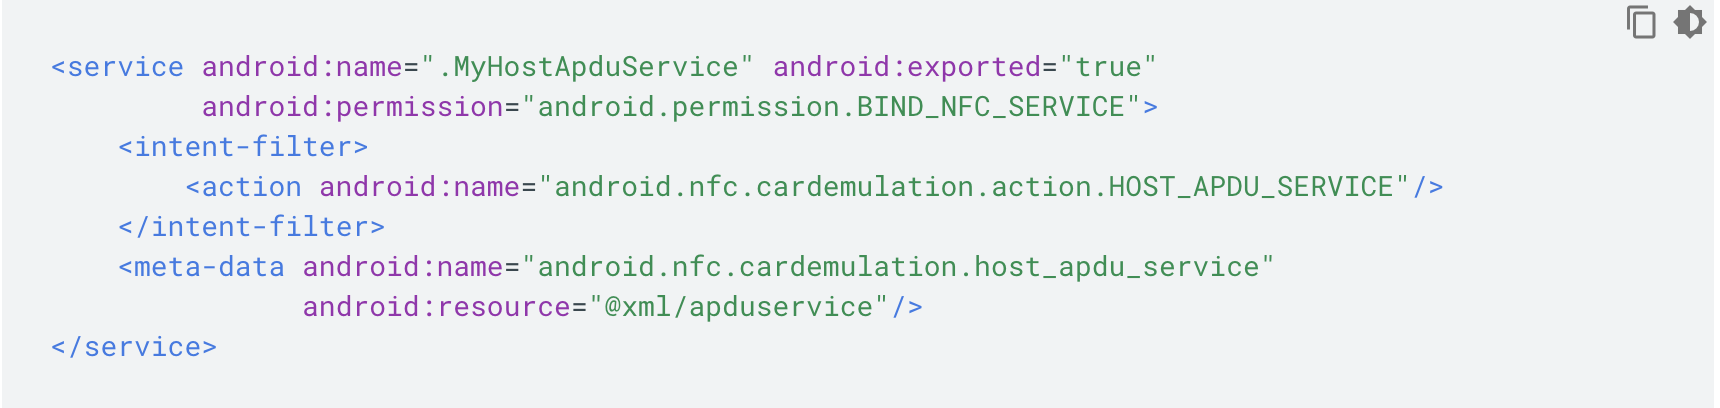
\includegraphics[width=\linewidth]
 	{img/ManifestService}
 	\caption{Service meta-data in AndroidManifest}
 	\label{fig:Manifest}
 \end{figure}

Bij het implementeren van de apdu service klasse wordt de klasse uitgebreid met de HostApduService klasse van android. De HostApduService klasse bevat twee abstracte methodes die overschreven worden in de eigen service klasse namelijk processCommandApdu en onDeactivated. De processCommandApdu methode wordt aangeroepen wanneer een NFC reader een APDU stuurt naar de apdu service en dan zal de service een APDU als antwoord terug sturen. Er moet wel rekening mee gehouden worden dat de processcommandApdu methode aangeroepen wordt op de main thread van de applicatie, wanneer het toestel dit niet aankan mag de main thread natuurlijk niet geblokkeerd worden. Wanneer de main thread het niet aankan moet de methode null teruggeven en een andere methode sendApduResponse die het antwoord op een andere thread terug zal sturen. De onDeactivated methode geeft terug of de apdu is teruggestuurd op de main thread of een andere thread wanneer de processCommandApdu wordt aangeroepen.

\section{Implementatie biometric factors}

Één van de beveiligingsmethodes die gekozen werd voor dit onderzoek zijn biometric factors, er zijn natuurlijk meerdere biometrische factoren die gebruikt kunnen worden om de applicatie te beveiligen zoals vingerscan, irisscan, spraak herkenning,... Hier werd gekozen voor de vingerscan te implementeren omdat dit een van de meest voorkomende beveiligingstechnologieën bij mobiele toestellen. Wanneer we een implementatie doen met vingerscan is het niet voldoende om enkel te vertrouwen op deze technologie of eender welke biometrische factor, het kan altijd voorkomen dat de technologie stopt met werken of de gekozen biometrische factor niet herkend wordt. Wanneer dit voorkomt moet er een back-up zijn, als back-up wordt er gekozen voor de pincode van het toestel te gebruiken ofwel en zelf ingestelde pincode voor de applicatie. Eerst en vooral moet er toestemming gegeven worden aan de applicatie om gebruik te maken van de vingerscan hardware van het mobiele toestel, dit gebeurt in de Android Manifest door middel van een metadata tag user-permission met de inhoud android:name="android.permission.USE\_FINGERPRINT. Voor de vingerscan implementatie moeten we twee extra klassen aangemaakt worden de FingerprintUiHelper klasse en de FingerprintAuthenticationoDialogFragement klasse. De FingerprintUiHelper klasse helpt om de tekst en de iconen te veranderen op de vingerscan authenticatie scherm. FingerprintAuthenticationDialogFragment communiceert met de vingerscan API om de gebruiker te authenticeren aan de hand van de vingerscan en als de vinger niet herkend wordtzal de authenticatie gebeuren aan de hand van de pincode. Bij het opstarten van de applicatie zal de vingerscan authenticatie scherm getoond worden vooraleer de gebruiker kan verder gaan en gebruik kan maken van de applicatie. 

\section{Implementatie encryption}

Bij de implementatie van encryption moeten er drie methodes toegevoegd worden aan de CardService die zorgen voor het encrypteren en het decrypteren van data respectievelijke encrypt, decrypt en generateKey. De generateKey functie genereert een unieke geheime sleutel die gebruikt wordt om data de encrypeteren. De encrypt functie maat gebruik van de generateKey functie om een sleutel te genereren die gebruikt zal worden samen met het geïnitialiseerde Cipher in ENCRYPT\_MODE om de data te encrypteren. Bij de decrypt funtie verloopt alles juist hetzelfde als bij de encrypt functie het enigste verschil is dat de Cipher geïnitialiseerd zal worden in DECRYPT\_MODE. Wanner de gebruiker zijn accountnummer ingeeft in de applicatie zal het nummer geëncrypteerd worden en opgeslagen worden, wanneer het accountnummmer getoond moet worden, zal het geëncrypteerde accountnummer weer gedecrypteerd worden. Wanneer een externe NFC-lezer de functie processCommandApdu aangeroep zal de geëncrypteerde data verstuurd worden en gedecrypteerd worden aan de kant van de NFC-lezer. Door de gegevens geëncrypteerd te versturen kan de data niet ontcijfert wanneer de data onderschept wordt door een aanvaller. De aanvaller kan de data enkel ontcijferen wanneer die in bezit is van de sleutel die gebruikt werd om de data te encrypteren ~\autocite{HowToEncrypt}. 

\section{Implementatie tokenization}

Tokenization wordt aanzien als een van de meest veilige vormen die geïmplementeerd kan worden in een betalingsapplicatie. Normaal gezien worden betalingstokens gegenereerd aan de kant van de backend waar het token gekoppeld wordt aan het de gebruiker die het token aanvraagt. Voor het doel van dit onderzoek was de implementatie van een volledig werkende backend overbodig en zal de functionaliteit nagebootst worden in de applicatie. Voor de functionaliteit na te bootsen implementeren we de functie nextToken die een nieuwe token genereerd die dan doorgestuurd kan worden in plaats van het accoutnummer. Iedere keer de processCommandApdu functie wordt aangeroepen door een externe NFC-lezer wordt de functie nextToken aangeroepen en wordt het nieuwe gegenereerde token doorgestuurd. Wanneer er gewerkt wordt met eenmalige tokens en een token wordt onderschept door een aanvaller kan de aanvaller hier niets mee aanvangen aangezien het token maar eenmalig gebruikt kan worden voor een transactie of autheticatie.

\section{Onderzoek}
\label{sec:onderzoek}

De grote vraag die nu gesteld kan worden is, welke beveiligingsmethode is nu de beste? Maar we moeten ons natuurlijk ook andere vragen stellen, is er maar één methode het veiligst? Zijn er meerdere methodes het veiligst? Kunnen sommige methodes gecombineerd worden? ... Om op al deze vragen een antwoord te kunnen geven zullen we de verschillende gekozen beveiligingsmethodes moeten vergelijken met elkaar. Het vergelijken van deze methodes kan op veel verschillende manieren gebeuren, we kunnen puur kijken naar de veiligheid van de methodes maar eigenlijk moeten we ook kijken naar de moeilijkheidsgraad van de implementatie. Niet iedere applicatie die gebruik wenst te maken van Host-based card emulation heeft een even hoge veiligheidsgraad nodig, zo kan een beveiligingsmethode te gecompliceerd zijn voor die specifieke use-case en heeft dit onderzoek niet veel nut. 

Wat zal er in dit onderzoek nu precies onderzocht worden? Er zal gekeken worden naar de moeilijkheidsgraad van de implementatie van de beveiligingsmethode, op welke momenten zijn de gevoelige gegevens zichtbaar, is de geïmplementeerde beveiligingsmethode gemakkelijk te omzeilen, is er een mogelijkheid om verschillende methodes te combineren, zorgt de combinatie van methodes voor extra veiligheid, is het overbodig om sommige methodes te combineren? Eenmaal we al deze vragen onderzocht hebben kan er een conclusie gemaakt worden over de verschillende methodes en kan u een geïnformeerde beslissing maken over welke implementatie het beste past voor uw specifieke use-case.